\documentclass[12pt]{article}
\usepackage{amsmath,amssymb,geometry,booktabs,array,mdframed,xcolor,enumitem,tikz}
\geometry{margin=0.85in}

\definecolor{purplemain}{RGB}{69,39,160}
\definecolor{purplelight}{RGB}{237,231,246}
\definecolor{teallight}{RGB}{224,242,241}
\definecolor{tealmain}{RGB}{0,105,92}
\definecolor{orangelight}{RGB}{255,243,224}
\definecolor{orangemain}{RGB}{230,81,0}
\definecolor{bluelight}{RGB}{227,242,253}
\definecolor{bluemain}{RGB}{21,101,192}

% Blank coordinate grid for student graphing
\newcommand{\blankgrid}{%
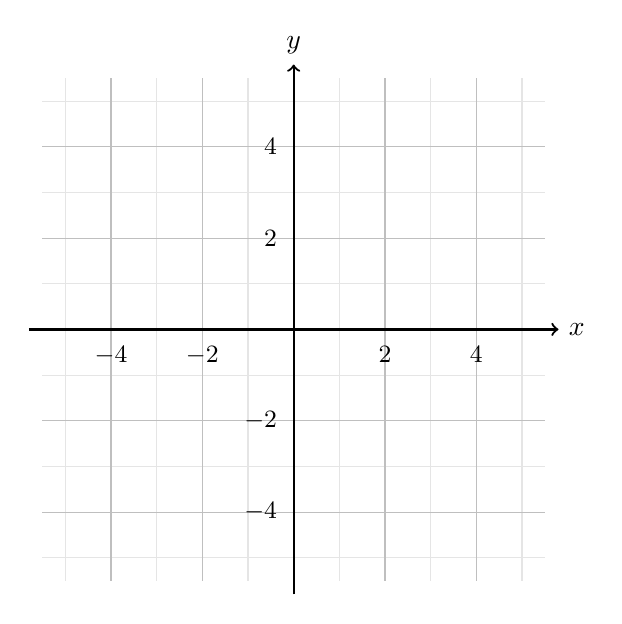
\begin{tikzpicture}[scale=0.58]
  \draw[step=1,gray!20,thin] (-5.5,-5.5) grid (5.5,5.5);
  \draw[step=2,gray!50] (-5.5,-5.5) grid (5.5,5.5);
  \draw[->,thick] (-5.8,0)--(5.8,0) node[right] {$x$};
  \draw[->,thick] (0,-5.8)--(0,5.8) node[above] {$y$};
  \foreach \x in {-4,-2,2,4} \node[below,font=\small] at (\x,-0.15) {$\x$};
  \foreach \y in {-4,-2,2,4} \node[left,font=\small]  at (-0.15,\y) {$\y$};
\end{tikzpicture}}

\begin{document}

%==================================================================
\begin{center}
  {\LARGE\textbf{Function Transformations}}\\[5pt]
  {\large Algebra 1 --- Shifts, Dilations, and Reflections}
\end{center}
\hrule\vspace{0.7em}

\section*{1. Translations (Shifts)}
\renewcommand{\arraystretch}{1.35}
\begin{center}
\begin{tabular}{lll}
\toprule
\textbf{Equation} & \textbf{Transformation} & \textbf{Point rule} \\
\midrule
$y=f(x)+k$ & Shift \textbf{up} $k$    & $(x,y)\to(x,\;y+k)$ \\
$y=f(x)-k$ & Shift \textbf{down} $k$  & $(x,y)\to(x,\;y-k)$ \\
$y=f(x-h)$ & Shift \textbf{right} $h$ & $(x,y)\to(x+h,\;y)$ \\
$y=f(x+h)$ & Shift \textbf{left} $h$  & $(x,y)\to(x-h,\;y)$ \\
\bottomrule
\end{tabular}
\end{center}

\section*{2. Dilations}
\begin{center}
\begin{tabular}{llll}
\toprule
\textbf{Form} & \textbf{Condition} & \textbf{Effect} & \textbf{Point rule}\\
\midrule
$y=a\,f(x)$ & $|a|>1$     & Vertical \textbf{stretch}       & $(x,y)\to(x,\;ay)$\\
$y=a\,f(x)$ & $0<|a|<1$   & Vertical \textbf{compression}   & $(x,y)\to(x,\;ay)$\\
$y=f(bx)$   & $|b|>1$     & Horizontal \textbf{compression} & $(x,y)\to(\frac{x}{b},\;y)$\\
$y=f(bx)$   & $0<|b|<1$   & Horizontal \textbf{stretch}     & $(x,y)\to(\frac{x}{b},\;y)$\\
\bottomrule
\end{tabular}
\end{center}

\section*{3. Reflections}
\begin{center}
\begin{tabular}{llll}
\toprule
\textbf{Equation} & \textbf{Reflection over} & \textbf{Point rule} & \textbf{Effect}\\
\midrule
$y=-f(x)$ & $x$-axis & $(x,y)\to(x,\;-y)$ & flip up/down\\
$y=f(-x)$ & $y$-axis & $(x,y)\to(-x,\;y)$ & flip left/right\\
\bottomrule
\end{tabular}
\end{center}

\begin{mdframed}[backgroundcolor=purplelight,linecolor=purplemain,linewidth=1pt,innerleftmargin=8pt]
\textbf{Memory rules:} Outside $f$ $\Rightarrow$ vertical change.\quad
Inside $f$ $\Rightarrow$ horizontal change (direction \textbf{opposite} to sign).\\
Negating \emph{outside} flips over $x$-axis.\quad Negating \emph{inside} flips over $y$-axis.
\end{mdframed}

\newpage
%==================================================================
\begin{center}{\LARGE\textbf{Practice Problems}}\end{center}
\hrule\vspace{0.5em}

%==================================================================
\begin{mdframed}[backgroundcolor=purplelight,linecolor=purplemain,linewidth=1.5pt,innerleftmargin=8pt]
{\large\textbf{Part A --- Translations}}
\end{mdframed}

%------ EXAMPLE --------------------------------------------------
\begin{mdframed}[backgroundcolor=purplelight!40,linecolor=purplemain,linewidth=0.8pt,innerleftmargin=8pt]
\textbf{Worked Example:}\quad Transform $y=x^2$ by shifting \textbf{right 2} and \textbf{up 1} to get $y=(x-2)^2+1$.

\vspace{0.4em}
\noindent
\begin{minipage}{0.52\textwidth}
\renewcommand{\arraystretch}{1.3}
\begin{tabular}{cc|cc}
\multicolumn{2}{c|}{\textbf{Parent } $y=x^2$} & \multicolumn{2}{c}{\textbf{New } $y=(x-2)^2+1$}\\
$x$ & $y$ & $x$ & $y$ \\\hline
$-2$ & $4$ & $0$ & $5$\\
$-1$ & $1$ & $1$ & $2$\\
$0$  & $0$ & $2$ & $1$ $\leftarrow$ vertex\\
$1$  & $1$ & $3$ & $2$\\
$2$  & $4$ & $4$ & $5$\\
\end{tabular}
\end{minipage}%
\begin{minipage}{0.48\textwidth}
\centering
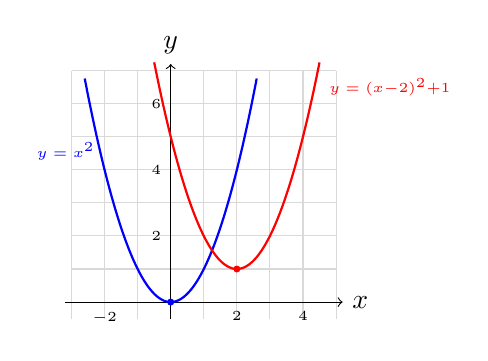
\begin{tikzpicture}[scale=0.42]
  \draw[step=1,gray!30,thin](-3,-0.5) grid (5,7);
  \draw[->](-3.2,0)--(5.2,0) node[right]{$x$};
  \draw[->](0,-0.5)--(0,7.2) node[above]{$y$};
  \foreach \x in {-2,2,4}\node[below,font=\tiny]at(\x,0){$\x$};
  \foreach \y in {2,4,6}\node[left,font=\tiny]at(0,\y){$\y$};
  \draw[blue,thick,domain=-2.6:2.6,smooth,variable=\x,samples=60] plot({\x},{(\x)^2});
  \draw[red,thick,domain=-0.5:4.5,smooth,variable=\x,samples=60] plot({\x},{(\x-2)^2+1});
  \filldraw[blue](0,0)circle(2.5pt); \filldraw[red](2,1)circle(2.5pt);
  \node[blue,font=\tiny,above left]at(-2,4){$y=x^2$};
  \node[red,font=\tiny,right]at(4.5,6.5){$y=(x{-}2)^2{+}1$};
\end{tikzpicture}
\end{minipage}
\end{mdframed}

\vspace{0.3em}
\begin{enumerate}[label=\textbf{A\arabic*.},leftmargin=*,itemsep=10pt]
\item Describe the transformation from $y=x^2$ to $y=x^2+5$.\vspace{1.6cm}
\item Describe the transformation from $y=x^2$ to $y=(x-3)^2$.\vspace{1.6cm}
\item Describe the transformation from $y=2^x$ to $y=2^x-4$.\vspace{1.6cm}
\item Describe the transformation from $y=2^x$ to $y=2^{x+1}$.\vspace{1.6cm}
\item Write the equation of $y=x^2$ shifted \textbf{left 2} and \textbf{down 3}.\vspace{1.6cm}
\item Write the equation of $y=2^x$ shifted \textbf{right 5} and \textbf{up 2}.\vspace{1.6cm}
\item The point $(3,9)$ lies on $y=x^2$. Find the corresponding point on $y=x^2+7$.\vspace{1.6cm}
\item The point $(2,4)$ lies on $y=x^2$. Find the corresponding point on $y=(x-1)^2$.\vspace{1.6cm}
\item Find the vertex of $y=(x-4)^2+3$.\vspace{1.6cm}
\item Find the horizontal asymptote of $y=2^x-6$.\vspace{1.2cm}
\end{enumerate}

\newpage
\noindent\textbf{\large Part A --- Multiple Choice (circle your answer)}
\vspace{0.5em}

\begin{enumerate}[label=\textbf{AM\arabic*.},leftmargin=*,itemsep=14pt]

\item Which point lies on $y=x^2+3$?\\[5pt]
\textbf{A.}\ $(0,0)$\qquad \textbf{B.}\ $(1,4)$\qquad \textbf{C.}\ $(2,4)$\qquad \textbf{D.}\ $(-1,2)$

\item The vertex of $y=(x+4)^2$ is at:\\[5pt]
\textbf{A.}\ $(4,0)$\qquad \textbf{B.}\ $(-4,0)$\qquad \textbf{C.}\ $(0,4)$\qquad \textbf{D.}\ $(0,-4)$

\item Which equation shifts $y=2^x$ right 3 units and down 1 unit?\\[5pt]
\textbf{A.}\ $y=2^{x+3}-1$\qquad \textbf{B.}\ $y=2^{x-3}+1$\qquad \textbf{C.}\ $y=2^{x-3}-1$\qquad \textbf{D.}\ $y=2^{x+3}+1$

\item The horizontal asymptote of $y=2^{x-2}+5$ is:\\[5pt]
\textbf{A.}\ $y=2$\qquad \textbf{B.}\ $y=-2$\qquad \textbf{C.}\ $y=5$\qquad \textbf{D.}\ $y=-5$

\item Which point rule describes a shift \textbf{down 4}?\\[5pt]
\textbf{A.}\ $(x,y)\to(x,y+4)$\qquad \textbf{B.}\ $(x,y)\to(x-4,y)$\qquad \textbf{C.}\ $(x,y)\to(x,y-4)$\qquad \textbf{D.}\ $(x,y)\to(x+4,y)$

\end{enumerate}

\vspace{0.8em}
\noindent\textbf{\large Part A --- Graph It!}
\vspace{0.4em}

\begin{enumerate}[label=\textbf{AG\arabic*.},leftmargin=*,itemsep=10pt]

\item On the axes below, plot at least 5 key points for $y=x^2$ (\textbf{blue}), then sketch $y=x^2-3$ (\textbf{red}) on the same axes. Label each curve and mark the vertex of each.

\vspace{0.4em}
\begin{center}\blankgrid\end{center}

\item On the axes below, sketch both $y=2^x$ (\textbf{blue}) and $y=2^{x+2}$ (\textbf{red}). Plot at least 4 points per curve. Label the $y$-intercept of each. State the horizontal asymptote.

\vspace{0.4em}
\begin{center}\blankgrid\end{center}
\textit{Asymptote: }\underline{\hspace{4cm}}

\end{enumerate}

\newpage
%==================================================================
\begin{mdframed}[backgroundcolor=bluelight,linecolor=bluemain,linewidth=1.5pt,innerleftmargin=8pt]
{\large\textbf{Part B --- Dilations}}
\end{mdframed}

%------ EXAMPLE --------------------------------------------------
\begin{mdframed}[backgroundcolor=bluelight!40,linecolor=bluemain,linewidth=0.8pt,innerleftmargin=8pt]
\textbf{Worked Example:}\quad Transform $y=x^2$ with a \textbf{vertical stretch by 2}: $y=2x^2$.

\vspace{0.4em}
\noindent
\begin{minipage}{0.52\textwidth}
\renewcommand{\arraystretch}{1.3}
\begin{tabular}{cc|c}
\multicolumn{2}{c|}{\textbf{Parent }$y=x^2$} & \textbf{New }$y=2x^2$\\
$x$ & $y$ & $y$\\\hline
$-2$ & $4$ & $8$\\
$-1$ & $1$ & $2$\\
$0$  & $0$ & $0$\\
$1$  & $1$ & $2$\\
$2$  & $4$ & $8$\\
\end{tabular}\\[4pt]
\small Point rule: $(x,y)\to(x,\,2y)$\\
Same vertex $(0,0)$; graph is \emph{narrower}.
\end{minipage}%
\begin{minipage}{0.48\textwidth}
\centering
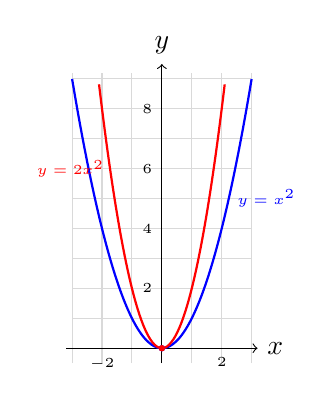
\begin{tikzpicture}[scale=0.38]
  \draw[step=1,gray!30,thin](-3,-0.5) grid (3,9.2);
  \draw[->](-3.2,0)--(3.2,0) node[right]{$x$};
  \draw[->](0,-0.5)--(0,9.5) node[above]{$y$};
  \foreach \x in {-2,2}\node[below,font=\tiny]at(\x,0){$\x$};
  \foreach \y in {2,4,6,8}\node[left,font=\tiny]at(0,\y){$\y$};
  \draw[blue,thick,domain=-3:3,smooth,variable=\x,samples=60] plot({\x},{(\x)^2});
  \draw[red,thick,domain=-2.1:2.1,smooth,variable=\x,samples=60] plot({\x},{2*(\x)^2});
  \filldraw[blue](0,0)circle(2.5pt); \filldraw[red](0,0)circle(2.5pt);
  \node[blue,font=\tiny,right]at(2.2,5){$y=x^2$};
  \node[red,font=\tiny,left]at(-1.6,6){$y=2x^2$};
\end{tikzpicture}
\end{minipage}
\end{mdframed}

\vspace{0.3em}
\begin{enumerate}[label=\textbf{B\arabic*.},leftmargin=*,itemsep=10pt]
\item Describe the transformation from $y=x^2$ to $y=5x^2$.\vspace{1.6cm}
\item Describe the transformation from $y=x^2$ to $y=\dfrac{1}{3}x^2$.\vspace{1.6cm}
\item Describe the transformation from $y=2^x$ to $y=4\cdot 2^x$.\vspace{1.6cm}
\item Describe the transformation from $y=2^x$ to $y=\dfrac{1}{4}\cdot 2^x$.\vspace{1.6cm}
\item The point $(2,4)$ lies on $y=x^2$. Find the corresponding point on $y=3x^2$.\vspace{1.6cm}
\item The point $(1,2)$ lies on $y=2^x$. Find the corresponding point on $y=\dfrac{1}{2}\cdot 2^x$.\vspace{1.6cm}
\item Describe the transformation from $y=x^2$ to $y=(3x)^2$.\vspace{1.6cm}
\item Describe the transformation from $y=2^x$ to $y=2^{2x}$.\vspace{1.6cm}
\item Write the equation for $y=x^2$ after a \textbf{vertical stretch by 6}.\vspace{1.6cm}
\item The point $(4,16)$ lies on $y=x^2$. After a horizontal compression by $\frac{1}{2}$, what is the new point?\vspace{1.2cm}
\end{enumerate}

\newpage
\noindent\textbf{\large Part B --- Multiple Choice (circle your answer)}
\vspace{0.5em}

\begin{enumerate}[label=\textbf{BM\arabic*.},leftmargin=*,itemsep=14pt]

\item Which equation is a \textbf{vertical stretch} of $y=x^2$ by a factor of 4?\\[5pt]
\textbf{A.}\ $y=\tfrac{x^2}{4}$\qquad \textbf{B.}\ $y=(4x)^2$\qquad \textbf{C.}\ $y=4x^2$\qquad \textbf{D.}\ $y=\left(\tfrac{x}{4}\right)^2$

\item The point $(3,9)$ on $y=x^2$ maps to which point on $y=\tfrac{1}{3}x^2$?\\[5pt]
\textbf{A.}\ $(3,3)$\qquad \textbf{B.}\ $(1,9)$\qquad \textbf{C.}\ $(9,9)$\qquad \textbf{D.}\ $(3,27)$

\item Which equation is a \textbf{horizontal stretch} of $y=2^x$ by a factor of 2?\\[5pt]
\textbf{A.}\ $y=2^{2x}$\qquad \textbf{B.}\ $y=2\cdot2^x$\qquad \textbf{C.}\ $y=2^{x/2}$\qquad \textbf{D.}\ $y=\tfrac{1}{2}\cdot2^x$

\item After a vertical compression by $\tfrac{1}{5}$, the point $(2,4)$ on $y=x^2$ becomes:\\[5pt]
\textbf{A.}\ $(10,4)$\qquad \textbf{B.}\ $(2,20)$\qquad \textbf{C.}\ $\left(2,\tfrac{4}{5}\right)$\qquad \textbf{D.}\ $\left(\tfrac{2}{5},4\right)$

\item The transformation $y=\left(\tfrac{1}{2}x\right)^2$ is best described as:\\[5pt]
\textbf{A.}\ Vertical compression by $\tfrac{1}{2}$\qquad \textbf{B.}\ Horizontal stretch by 2\\[3pt]
\textbf{C.}\ Vertical stretch by 2\qquad \textbf{D.}\ Horizontal compression by $\tfrac{1}{2}$

\end{enumerate}

\vspace{0.8em}
\noindent\textbf{\large Part B --- Graph It!}
\vspace{0.4em}

\begin{enumerate}[label=\textbf{BG\arabic*.},leftmargin=*,itemsep=10pt]

\item On the axes below, plot $y=x^2$ (\textbf{blue}) and $y=\tfrac{1}{2}x^2$ (\textbf{red}) using at least 5 key points each. How do the two graphs compare in width?

\vspace{0.4em}
\begin{center}\blankgrid\end{center}
\textit{Comparison: }\underline{\hspace{8cm}}

\item On the axes below, sketch $y=2^x$ (\textbf{blue}) and $y=3\cdot2^x$ (\textbf{red}) using at least 4 points each. Label the $y$-intercept of each curve.

\vspace{0.4em}
\begin{center}\blankgrid\end{center}

\end{enumerate}

\newpage
%==================================================================
\begin{mdframed}[backgroundcolor=teallight,linecolor=tealmain,linewidth=1.5pt,innerleftmargin=8pt]
{\large\textbf{Part C --- Reflections}}
\end{mdframed}

%------ EXAMPLE --------------------------------------------------
\begin{mdframed}[backgroundcolor=teallight!50,linecolor=tealmain,linewidth=0.8pt,innerleftmargin=8pt]
\textbf{Worked Example:}\quad Reflect $y=2^x$ over the $x$-axis to get $y=-2^x$.

\vspace{0.4em}
\noindent
\begin{minipage}{0.52\textwidth}
\renewcommand{\arraystretch}{1.3}
\begin{tabular}{cc|c}
\multicolumn{2}{c|}{\textbf{Parent }$y=2^x$} & \textbf{New }$y=-2^x$\\
$x$ & $y$ & $y$\\\hline
$-2$ & $\tfrac{1}{4}$ & $-\tfrac{1}{4}$\\
$-1$ & $\tfrac{1}{2}$ & $-\tfrac{1}{2}$\\
$0$  & $1$            & $-1$\\
$1$  & $2$            & $-2$\\
$2$  & $4$            & $-4$\\
\end{tabular}\\[4pt]
\small Point rule: $(x,y)\to(x,-y)$\\
Asymptote stays $y=0$; graph flips down.
\end{minipage}%
\begin{minipage}{0.48\textwidth}
\centering
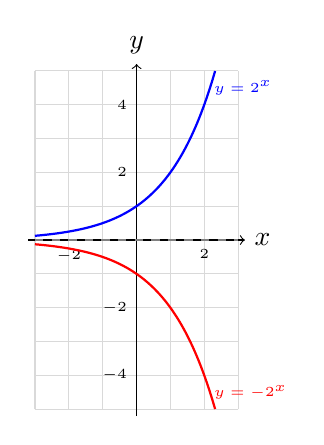
\begin{tikzpicture}[scale=0.43]
  \draw[step=1,gray!30,thin](-3,-5) grid (3,5);
  \draw[->](-3.2,0)--(3.2,0) node[right]{$x$};
  \draw[->](0,-5.2)--(0,5.2) node[above]{$y$};
  \foreach \x in {-2,2}\node[below,font=\tiny]at(\x,0){$\x$};
  \foreach \y in {-4,-2,2,4}\node[left,font=\tiny]at(0,\y){$\y$};
  \draw[blue,thick,domain=-3:2.32,smooth,variable=\x,samples=60] plot({\x},{exp(\x*0.6931)});
  \draw[red,thick,domain=-3:2.32,smooth,variable=\x,samples=60] plot({\x},{-exp(\x*0.6931)});
  \draw[gray,dashed,thin](-3,0)--(3,0);
  \node[blue,font=\tiny,right]at(2,4.5){$y=2^x$};
  \node[red,font=\tiny,right]at(2,-4.5){$y=-2^x$};
\end{tikzpicture}
\end{minipage}
\end{mdframed}

\vspace{0.3em}
\begin{enumerate}[label=\textbf{C\arabic*.},leftmargin=*,itemsep=10pt]
\item Describe the transformation from $y=x^2$ to $y=-x^2$.\vspace{1.6cm}
\item Is $y=(-x)^2$ the same as $y=x^2$? Explain.\vspace{1.6cm}
\item Describe the transformation from $y=2^x$ to $y=-2^x$.\vspace{1.6cm}
\item Describe $y=2^{-x}$. Is this function increasing or decreasing?\vspace{1.6cm}
\item The point $(2,4)$ lies on $y=x^2$. Find the corresponding point on $y=-x^2$.\vspace{1.6cm}
\item The point $(1,2)$ lies on $y=2^x$. Find the corresponding point on $y=2^{-x}$.\vspace{1.6cm}
\item The point $(-3,9)$ lies on $y=x^2$. Find its image after reflecting over the $x$-axis.\vspace{1.6cm}
\item Write the equation for $y=2^x$ reflected over the $y$-axis.\vspace{1.6cm}
\item Write the equation for $y=x^2-3$ reflected over the $x$-axis. Simplify.\vspace{1.6cm}
\item List \textbf{all} transformations applied to $y=x^2$ to obtain $y=-(x+2)^2+1$. State the correct order.\vspace{1.6cm}
\end{enumerate}

\newpage
\noindent\textbf{\large Part C --- Multiple Choice (circle your answer)}
\vspace{0.5em}

\begin{enumerate}[label=\textbf{CM\arabic*.},leftmargin=*,itemsep=14pt]

\item The reflection of the point $(3,9)$ over the $x$-axis is:\\[5pt]
\textbf{A.}\ $(-3,9)$\qquad \textbf{B.}\ $(3,-9)$\qquad \textbf{C.}\ $(-3,-9)$\qquad \textbf{D.}\ $(9,3)$

\item Which equation reflects $y=x^2-4$ over the $x$-axis?\\[5pt]
\textbf{A.}\ $y=-x^2+4$\qquad \textbf{B.}\ $y=x^2+4$\qquad \textbf{C.}\ $y=(-x)^2-4$\qquad \textbf{D.}\ $y=-x^2-4$

\item After reflecting $y=2^x$ over the $y$-axis, what is the new $y$-intercept?\\[5pt]
\textbf{A.}\ $(0,-1)$\qquad \textbf{B.}\ $(0,0)$\qquad \textbf{C.}\ $(0,2)$\qquad \textbf{D.}\ $(0,1)$

\item Which equation reflects $y=2^{x-1}+3$ over the $x$-axis?\\[5pt]
\textbf{A.}\ $y=-2^{x-1}+3$\qquad \textbf{B.}\ $y=-2^{x-1}-3$\qquad \textbf{C.}\ $y=2^{-(x-1)}+3$\qquad \textbf{D.}\ $y=2^{-x-1}+3$

\item Which statement about $y=(-x)^2$ is true?\\[5pt]
\textbf{A.}\ It equals $-x^2$\qquad \textbf{B.}\ It equals $x^2$\qquad \textbf{C.}\ It opens downward\qquad \textbf{D.}\ Its vertex is $(-1,0)$

\end{enumerate}

\vspace{0.8em}
\noindent\textbf{\large Part C --- Graph It!}
\vspace{0.4em}

\begin{enumerate}[label=\textbf{CG\arabic*.},leftmargin=*,itemsep=10pt]

\item On the axes below, graph $y=x^2$ (\textbf{blue}) and $y=-x^2$ (\textbf{red}) using at least 5 key points each. Describe the relationship between the two curves.

\vspace{0.4em}
\begin{center}\blankgrid\end{center}
\textit{Relationship: }\underline{\hspace{8cm}}

\item On the axes below, sketch $y=2^x$ (\textbf{blue}) and $y=2^{-x}$ (\textbf{red}). Plot at least 4 points per curve. What is the same about both graphs? What is different?

\vspace{0.4em}
\begin{center}\blankgrid\end{center}
\textit{Same: }\underline{\hspace{5cm}}\quad\textit{Different: }\underline{\hspace{5cm}}

\end{enumerate}

\newpage
%==================================================================
\begin{mdframed}[backgroundcolor=orangelight,linecolor=orangemain,linewidth=1.5pt,innerleftmargin=8pt]
{\large\textbf{Part D --- Combined Transformations (Multiple Choice)}}
\end{mdframed}

\begin{enumerate}[label=\textbf{D\arabic*.},leftmargin=*,itemsep=16pt]

\item Which equation represents $y=x^2$ shifted \textbf{right 3}, vertically \textbf{stretched by 2}, and shifted \textbf{up 1}?\\[5pt]
\textbf{A.}\ $y=2(x+3)^2+1$\quad \textbf{B.}\ $y=2(x-3)^2+1$\quad \textbf{C.}\ $y=2(x-3)^2-1$\quad \textbf{D.}\ $y=\tfrac{1}{2}(x-3)^2+1$

\item The point $(1,2)$ on $y=2^x$, after reflecting over the $x$-axis then shifting \textbf{up 3}, becomes:\\[5pt]
\textbf{A.}\ $(1,1)$\qquad \textbf{B.}\ $(-1,5)$\qquad \textbf{C.}\ $(1,5)$\qquad \textbf{D.}\ $(1,-5)$

\item Which equation is a \textbf{vertical compression} of $y=x^2$ by $\tfrac{1}{4}$?\\[5pt]
\textbf{A.}\ $y=4x^2$\qquad \textbf{B.}\ $y=(4x)^2$\qquad \textbf{C.}\ $y=\tfrac{1}{4}x^2$\qquad \textbf{D.}\ $y=\left(\tfrac{1}{4}x\right)^2$

\item The horizontal asymptote of $y=3\cdot2^{x+2}-5$ is:\\[5pt]
\textbf{A.}\ $y=3$\qquad \textbf{B.}\ $y=2$\qquad \textbf{C.}\ $y=-5$\qquad \textbf{D.}\ $y=5$

\item Which correctly describes all transformations of $y=-2(x-1)^2+4$?\\[5pt]
\textbf{A.}\ Shift left 1, stretch 2, reflect $x$-axis, up 4\qquad \textbf{B.}\ Shift right 1, stretch 2, reflect $x$-axis, up 4\\[3pt]
\textbf{C.}\ Shift right 1, compress 2, reflect $x$-axis, down 4\qquad \textbf{D.}\ Shift right 1, stretch 2, up 4

\item The point $(3,8)$ on $y=2^x$, after the transformation $y=-2^x+5$, becomes:\\[5pt]
\textbf{A.}\ $(3,-3)$\qquad \textbf{B.}\ $(-3,-3)$\qquad \textbf{C.}\ $(3,13)$\qquad \textbf{D.}\ $(3,3)$

\item The vertex of $y=-3(x+2)^2-1$ is:\\[5pt]
\textbf{A.}\ $(2,-1)$\qquad \textbf{B.}\ $(-2,-1)$\qquad \textbf{C.}\ $(2,1)$\qquad \textbf{D.}\ $(-2,1)$

\item Which equation represents $y=2^x$ reflected over the $y$-axis, then shifted up 3?\\[5pt]
\textbf{A.}\ $y=-2^x+3$\qquad \textbf{B.}\ $y=2^{-x}-3$\qquad \textbf{C.}\ $y=2^{-x}+3$\qquad \textbf{D.}\ $y=-2^{-x}+3$

\item The point $(6,36)$ on $y=x^2$, after a horizontal compression by $\tfrac{1}{3}$, becomes:\\[5pt]
\textbf{A.}\ $(6,12)$\qquad \textbf{B.}\ $(18,36)$\qquad \textbf{C.}\ $(2,36)$\qquad \textbf{D.}\ $(2,12)$

\item Which equation has vertex $(-1,5)$, opens \textbf{downward}, and is \textbf{narrower} than $y=x^2$?\\[5pt]
\textbf{A.}\ $y=2(x-1)^2+5$\quad \textbf{B.}\ $y=-2(x+1)^2+5$\quad \textbf{C.}\ $y=-\tfrac{1}{2}(x+1)^2+5$\quad \textbf{D.}\ $y=2(x+1)^2-5$

\end{enumerate}

\newpage
%==================================================================
\begin{center}{\LARGE\textbf{Answer Key}}\end{center}
\hrule\vspace{0.7em}

\begin{mdframed}[backgroundcolor=purplelight,linecolor=purplemain,linewidth=1.2pt,innerleftmargin=8pt]
{\large\textbf{Part A --- Translations}}
\end{mdframed}
\begin{enumerate}[label=\textbf{A\arabic*.},leftmargin=*,itemsep=4pt]
\item Shift \textbf{up 5 units}. $(x,y)\to(x,y+5)$.
\item Shift \textbf{right 3 units}. $(x,y)\to(x+3,y)$.
\item Shift \textbf{down 4 units}. Asymptote moves to $y=-4$.
\item Shift \textbf{left 1 unit}. Asymptote stays $y=0$.
\item $y=(x+2)^2-3$\quad (vertex at $(-2,-3)$).
\item $y=2^{x-5}+2$\quad (asymptote: $y=2$; $y$-int: $(0,\tfrac{1}{32}+2)$).
\item $(3,16)$\quad --- $y$ increases by 7: $9+7=16$.
\item $(3,4)$\quad --- $x$ shifts right 1: $x=3$, $y=(3-1)^2=4$.
\item Vertex: $(4,3)$.
\item Asymptote: $y=-6$.
\end{enumerate}

\noindent\textbf{Part A MC:}\quad AM1: \textbf{B}\quad AM2: \textbf{B}\quad AM3: \textbf{C}\quad AM4: \textbf{C}\quad AM5: \textbf{C}

\noindent\textit{Part A Graphing:}
\begin{itemize}[itemsep=2pt]
\item \textbf{AG1:} $y=x^2$ vertex $(0,0)$; $y=x^2-3$ vertex $(0,-3)$, same shape, shifted down 3.
\item \textbf{AG2:} $y=2^x$ has $y$-int $(0,1)$; $y=2^{x+2}$ has $y$-int $(0,4)$ (shifted left 2). Both: asymptote $y=0$.
\end{itemize}

\vspace{0.5em}
\begin{mdframed}[backgroundcolor=bluelight,linecolor=bluemain,linewidth=1.2pt,innerleftmargin=8pt]
{\large\textbf{Part B --- Dilations}}
\end{mdframed}
\begin{enumerate}[label=\textbf{B\arabic*.},leftmargin=*,itemsep=4pt]
\item Vertical \textbf{stretch} by factor 5 (graph narrower). $(x,y)\to(x,5y)$.
\item Vertical \textbf{compression} by factor $\tfrac{1}{3}$ (graph wider).
\item Vertical \textbf{stretch} by factor 4. $y$-int moves from $(0,1)$ to $(0,4)$.
\item Vertical \textbf{compression} by factor $\tfrac{1}{4}$. $y$-int: $(0,\tfrac{1}{4})$.
\item $(2,12)$\quad $y$-value $\times3$: $4\times3=12$.
\item $(1,1)$\quad $y$-value $\times\tfrac{1}{2}$: $2\times\tfrac{1}{2}=1$.
\item Horizontal \textbf{compression} by $\tfrac{1}{3}$ (same as vertical stretch by 9, since $(3x)^2=9x^2$).
\item Horizontal \textbf{compression} by $\tfrac{1}{2}$. $(x,y)\to(\tfrac{x}{2},y)$.
\item $y=6x^2$.
\item $(2,16)$\quad $x\div2=2$, $y$ unchanged.
\end{enumerate}

\noindent\textbf{Part B MC:}\quad BM1: \textbf{C}\quad BM2: \textbf{A}\quad BM3: \textbf{C}\quad BM4: \textbf{C}\quad BM5: \textbf{B}

\noindent\textit{Part B Graphing:}
\begin{itemize}[itemsep=2pt]
\item \textbf{BG1:} $y=x^2$ is \emph{wider}; $y=\tfrac{1}{2}x^2$ is \emph{wider} than $y=x^2$. Both share vertex $(0,0)$.
\item \textbf{BG2:} $y=2^x$: $y$-int $(0,1)$;\quad $y=3\cdot2^x$: $y$-int $(0,3)$. Second is a vertical stretch; grows faster.
\end{itemize}

\vspace{0.5em}
\begin{mdframed}[backgroundcolor=teallight,linecolor=tealmain,linewidth=1.2pt,innerleftmargin=8pt]
{\large\textbf{Part C --- Reflections}}
\end{mdframed}
\begin{enumerate}[label=\textbf{C\arabic*.},leftmargin=*,itemsep=4pt]
\item Reflection over the \textbf{$x$-axis}; graph opens downward. $(x,y)\to(x,-y)$.
\item \textbf{Yes, same graph.} $(-x)^2=x^2$ --- parabola is an even function.
\item Reflection over the \textbf{$x$-axis}; graph is below the $x$-axis; asymptote stays $y=0$.
\item Reflection over the \textbf{$y$-axis}. The function is \textbf{decreasing} (as $x$ increases, $2^{-x}$ decreases).
\item $(2,-4)$\quad negate $y$: $4\to-4$.
\item $(-1,2)$\quad negate $x$: $1\to-1$.
\item $(-3,-9)$ on $y=-x^2$.
\item $y=2^{-x}$.
\item $y=-(x^2-3)=-x^2+3$.
\item Order: \textbf{(1)} shift left 2, \textbf{(2)} reflect over $x$-axis, \textbf{(3)} shift up 1.
\end{enumerate}

\noindent\textbf{Part C MC:}\quad CM1: \textbf{B}\quad CM2: \textbf{A}\quad CM3: \textbf{D}\quad CM4: \textbf{B}\quad CM5: \textbf{B}

\noindent\textit{Part C Graphing:}
\begin{itemize}[itemsep=2pt]
\item \textbf{CG1:} $y=-x^2$ is a mirror image of $y=x^2$ reflected over the $x$-axis. Same shape, opens down.
\item \textbf{CG2:} Same: both have $y$-int $(0,1)$ and asymptote $y=0$. Different: $y=2^x$ increases, $y=2^{-x}$ decreases. They are mirror images over the $y$-axis.
\end{itemize}

\vspace{0.5em}
\begin{mdframed}[backgroundcolor=orangelight,linecolor=orangemain,linewidth=1.2pt,innerleftmargin=8pt]
{\large\textbf{Part D --- Combined MC}}
\end{mdframed}
\noindent\textbf{D1: B}\quad\textbf{D2: A}\quad\textbf{D3: C}\quad\textbf{D4: C}\quad\textbf{D5: B}\quad\textbf{D6: A}\quad\textbf{D7: B}\quad\textbf{D8: C}\quad\textbf{D9: C}\quad\textbf{D10: B}

\vspace{0.5em}
\noindent\textit{Selected explanations:}
\begin{itemize}[itemsep=2pt]
\item D2: Reflect $(1,2)\to(1,-2)$; shift up 3: $-2+3=1$. New point $(1,1)$.
\item D4: Only the $-5$ outside shifts the asymptote from $y=0$ to $y=-5$.
\item D6: $-2^3+5=-8+5=-3$. New point $(3,-3)$.
\item D9: Horiz.\ compression by $\tfrac{1}{3}$: $x\to\tfrac{x}{3}=\tfrac{6}{3}=2$, $y$ unchanged. Point $(2,36)$.
\end{itemize}

\end{document}
